\section{Game Setup}

The Barbarian player starts with control of the Helvetii tribe at full strength in its home area, as well as all German units at full strength in Germania. Stand these units up, facing the Barbarian player.

The Roman player starts with six Roman legions in Transalpine Gaul - legions VII, VIII, IX, and X (Caesar) at full strength, as well as legions XI and XII at strength 3 each. The Roman player also controls the Volcae tribe at full strength in its home area, and the Allobroges tribe at strength 1 in its home area. Stand these units up, facing the Roman player.

\begin{figure}[h]
  \centering
  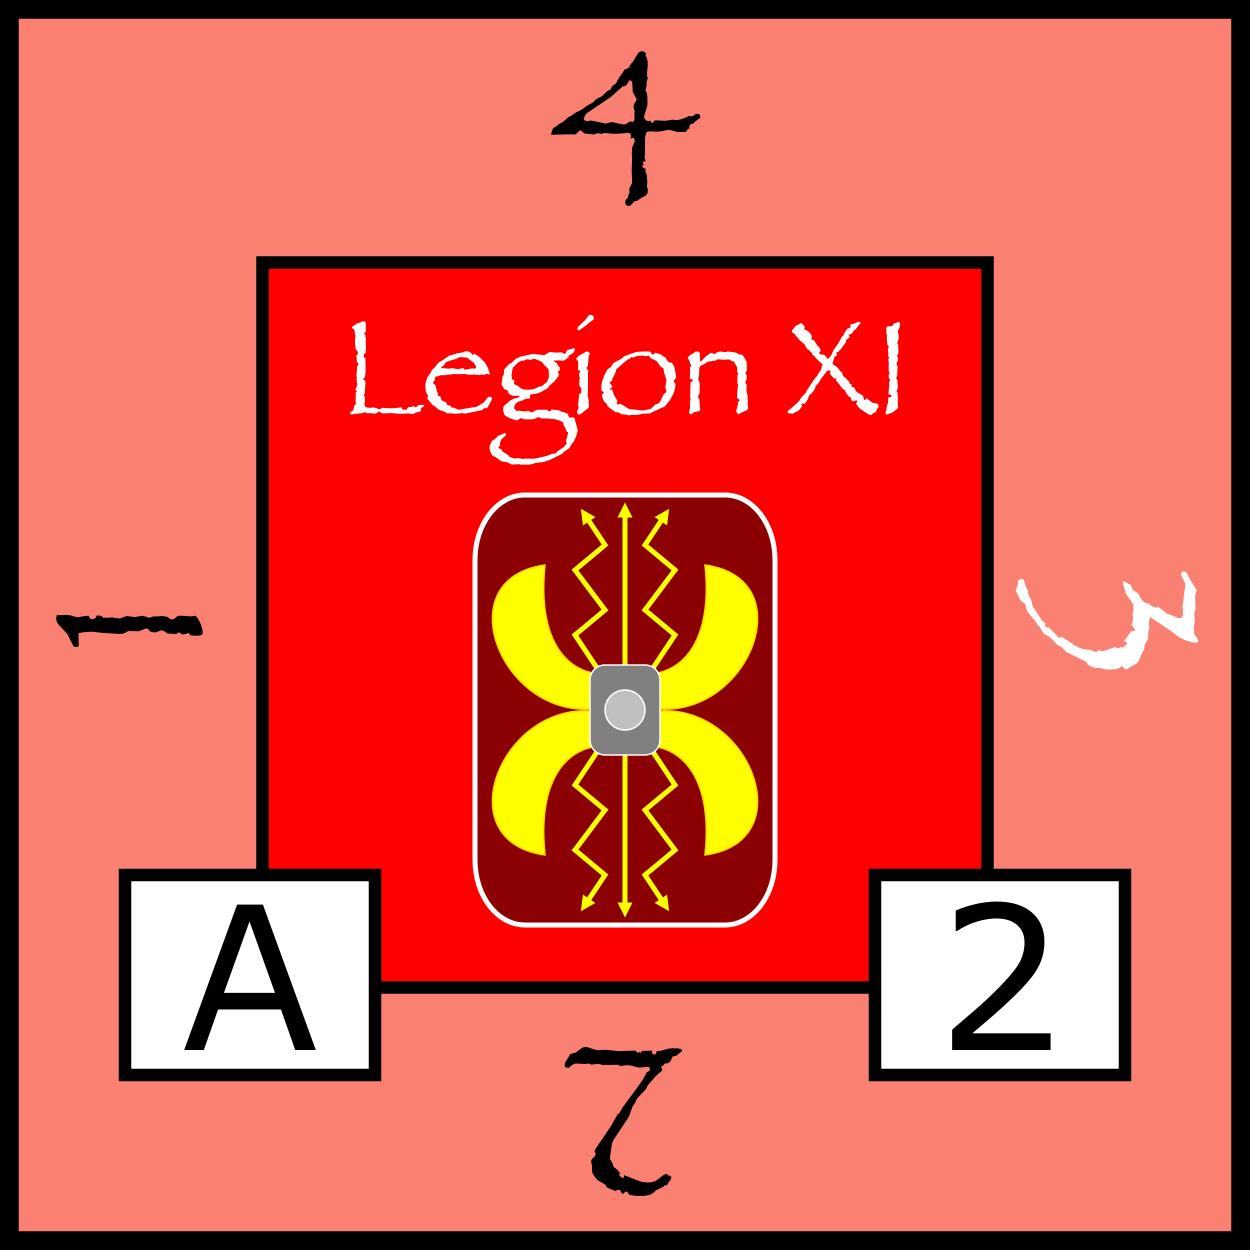
\includegraphics[width=0.25\linewidth, angle=90]{Legion_XI.png}
  \hspace{10mm}
  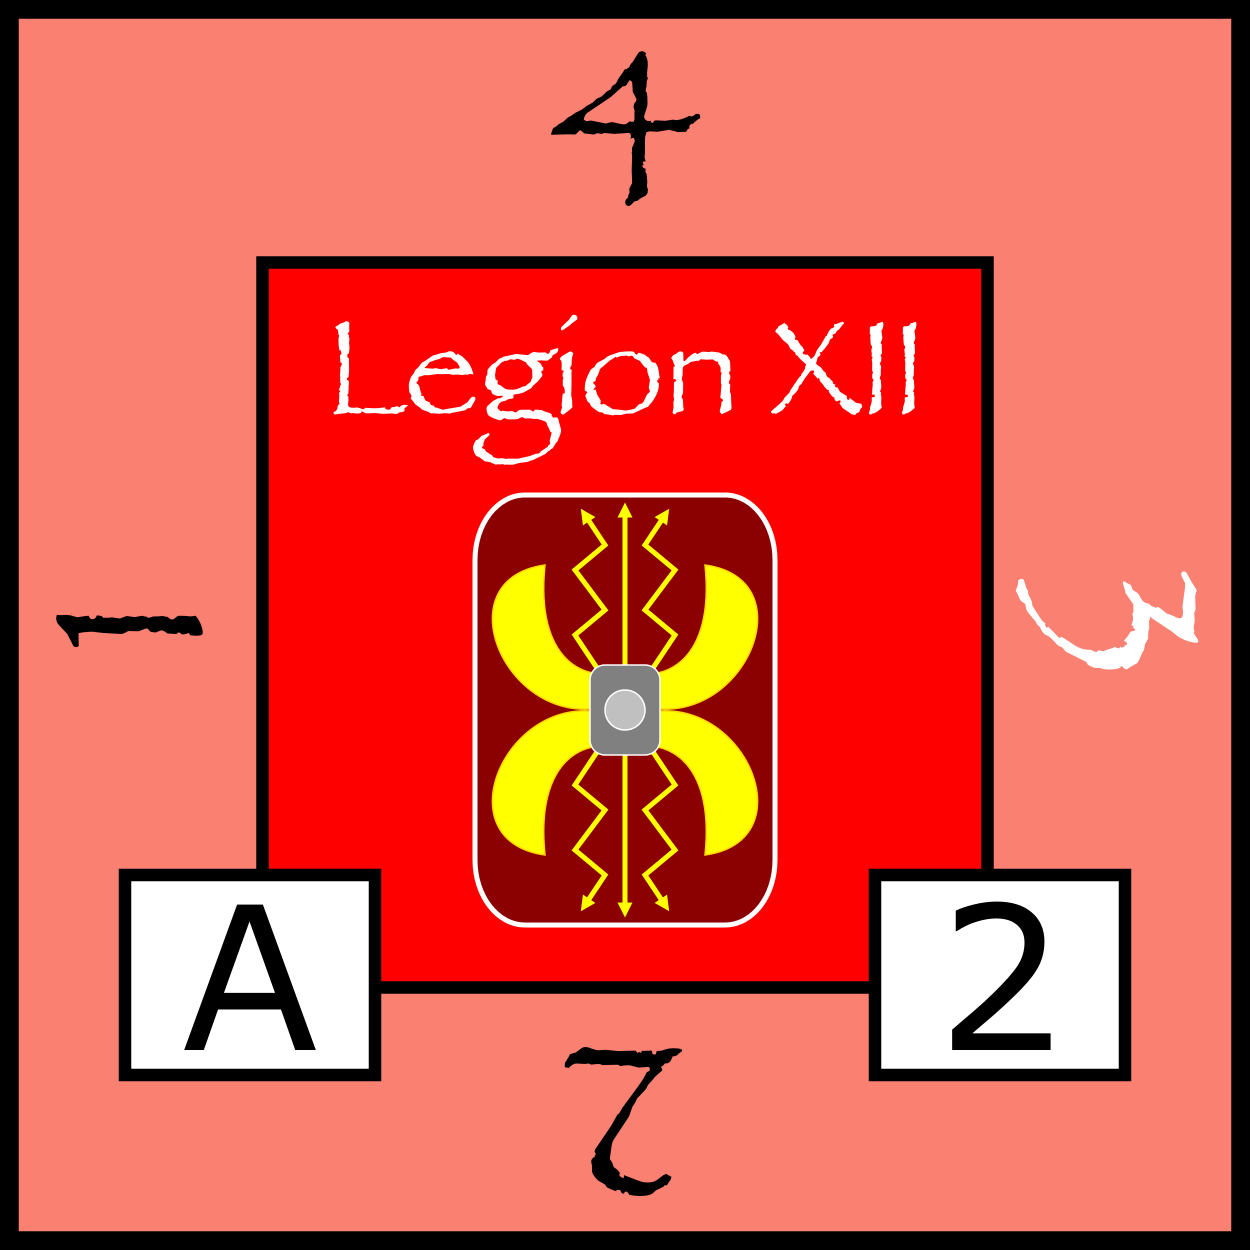
\includegraphics[width=0.25\linewidth, angle=90]{Legion_XII.png}
  \caption*{Legions XI and XII}
\end{figure}

\textit{Legions XI and XII had been recruited shortly before Caesar began his campaign and so their strength has been reduced to represent their lack of experience. Historically Caesar used them in a reserve capacity the first year. (Book I, Chapter 24)}

The Roman player starts with 15 supply points. Use the provided markers on the general records track supply points throughout the game.

All other Gallic tribes are placed face down in their home areas. They begin the game neutral. As these units become active, they should be stood upright, with the label facing the controlling player.

There are several Gallic areas that list two tribes as their home area. If the names are separated by a slash, such as "Menapi / Nervii" then only one of those tribes will start the game in play. Randomly select one of the tribes for that home area, and set aside the other tribe for now. Both players may know which tribe was selected, and while still neutral it can be inspected if you forget. If the names are separated by a plus sign such as "Bellovaci + Caletes", then both blocks are placed in that area and treat that space as their home area.

The following is a list of variable tribes that players should roll for at the start of the game.

\begin{itemize}[nosep]
  \item Atrebates or Morini
  \item Carnutes or Cenomani
  \item Esuvii or Luxovii
  \item Menapi or Nervii
  \item Pictones or Namnetes
  \item Remi or Atuatuci
  \item Tarbelli or Elusates
  \item Tolosates or Sotiates
\end{itemize}